\documentclass[
    12pt,
    oneside,
    a4paper,
    english,
    brazilian,
    chapter=TITLE,
    sumario=tradicional
]{abntex2}

\usepackage[utf8]{inputenc}
\usepackage[T1]{fontenc}
\usepackage{times}
\usepackage{microtype}
\usepackage{indentfirst}
\usepackage{graphicx}
\usepackage{amsmath,amssymb}
\usepackage{float}
\usepackage{xcolor}
\usepackage{textcomp}
\usepackage{listings}
\usepackage{xurl}
\hypersetup{
    colorlinks=false,
    pdfborder={0 0 0},
    hypertexnames=false,
    pdftitle={Métodos Numéricos para Equações Diferenciais II - Trabalho 1},
    pdfauthor={Kauan Peçanha Lira}
}

\graphicspath{{figures/}{./}}

\setlrmarginsandblock{3cm}{2cm}{*}
\setulmarginsandblock{3cm}{2cm}{*}
\checkandfixthelayout
\setlength{\parindent}{1.3cm}
\setlength{\parskip}{0pt}
\OnehalfSpacing

\renewcommand{\ABNTEXchapterfont}{\normalfont\bfseries}
\renewcommand{\ABNTEXchapterfontsize}{\normalsize}
\renewcommand{\ABNTEXsectionfont}{\normalfont\bfseries}
\renewcommand{\ABNTEXsectionfontsize}{\normalsize}
\renewcommand{\ABNTEXsubsectionfont}{\normalfont\bfseries}
\renewcommand{\ABNTEXsubsectionfontsize}{\normalsize}

\setlength{\beforechapskip}{0pt}
\setlength{\afterchapskip}{1.5\baselineskip}

\newcommand{\nomedainstituicao}{UNIVERSIDADE DO ESTADO DO RIO DE JANEIRO}
\newcommand{\nomedaunidade}{INSTITUTO POLITÉCNICO}
\newcommand{\nomedocurso}{GRADUAÇÃO EM ENGENHARIA DE COMPUTAÇÃO}

\titulo{Métodos Numéricos para Equações Diferenciais II\\Trabalho 1}
\autor{Kauan Peçanha Lira}
\local{Nova Friburgo}
\data{2026}
\tipotrabalho{Trabalho acadêmico}
\preambulo{Trabalho apresentado à disciplina de Métodos Numéricos para
Equações Diferenciais II, do curso de Engenharia de Computação do Instituto
Politécnico da Universidade do Estado do Rio de Janeiro.}

\lstset{
    language=Python,
    basicstyle=\ttfamily\small,
    keywordstyle=\color{blue},
    commentstyle=\color{gray},
    stringstyle=\color{teal},
    numbers=left,
    numberstyle=\tiny,
    frame=single,
    breaklines=true,
    showstringspaces=false,
    literate={°}{{\textdegree}}1
}

\begin{document}
\selectlanguage{brazilian}
\frenchspacing

\begin{titlingpage}
    \begin{center}
        \begin{minipage}{0.18\textwidth}
            \centering
            
\includegraphics[width=2.2cm]{uerj.png}
        \end{minipage}%
        \begin{minipage}{0.62\textwidth}
            \centering
            \textbf{\nomedainstituicao}\\
            \rule{7cm}{0.4pt}\\
            \textbf{\nomedaunidade\\\nomedocurso}
        \end{minipage}%
        \begin{minipage}{0.18\textwidth}
            \centering
            
\includegraphics[width=2.8cm]{iprj.jpeg}
        \end{minipage}

        \vspace*{4cm}
        {\bfseries\large\imprimirautor\par}
        \vspace*{3cm}
        {\bfseries\large\imprimirtitulo\par}
        \vfill
        {\bfseries\large\imprimirlocal\\\imprimirdata\par}
    \end{center}
\end{titlingpage}

\begin{titlingpage}
    \begin{center}
        {\imprimirautor\par}
        \vspace*{\fill}
        {\bfseries\imprimirtitulo\par}
        \vspace*{\fill}
        \hspace{0.45\textwidth}
        \begin{minipage}{0.5\textwidth}
            \SingleSpacing
            \imprimirpreambulo

            \vspace{0.8cm}
            Matrícula: 202110048911.
        \end{minipage}\par
        \vspace*{\fill}
        {\imprimirlocal\\\imprimirdata\par}
    \end{center}
\end{titlingpage}

\pdfbookmark[0]{\contentsname}{toc}
\tableofcontents*
\cleardoublepage

\textual

\chapter{Lista 1 -- Questão 1}

\section{Enunciado}

Seja uma placa metálica que foi submetida ao aquecimento uniforme e encontra-se
no regime estacionário. A influência da espessura na propagação térmica foi
considerada nula, por ser diminuta em comparação com as outras dimensões.

Realize a discretização da malha de cálculo utilizando o princípio do Método
das diferenças finitas para as seguintes situações.

\[
    \frac{\partial ^ 2 T}{\partial x ^ 2} + \frac{\partial ^ 2 T}{\partial y ^ 2} = 0
\]

\[
    H = L = 0{,}1\,\mathrm{m}
\]

\[
    T_{\infty} = 10\,^\circ\mathrm{C}
\]

\[
    K = 150\,\frac{\mathrm{W}}{\mathrm{m}\cdot\mathrm{K}}
\]

\[
    h = 450\,\frac{\mathrm{W}}{\mathrm{m}^2\cdot\mathrm{K}}
\]

\[
    \text{Erro} = 1\%
\]

\[
    N_x = N_y = 10
\]

\begin{figure}[H]
    \centering
    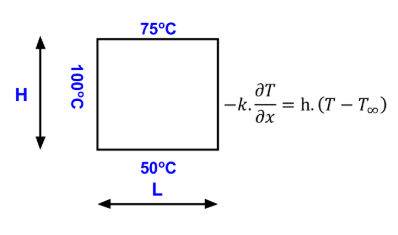
\includegraphics[width=0.4\linewidth]{lista1-questao1.png}
    \caption{Configuração da placa metálica}
    \label{fig:lista1-configuracao}

    {\small Fonte: slides do professor.\par}
\end{figure}

\newpage

\section{Solução}

% 

Em regime estacionário e sem geração interna de calor, a temperatura na placa
é regida pela equação de Laplace:

\[
    \frac{\partial^2 T}{\partial x^2}
    +
    \frac{\partial^2 T}{\partial y^2}
    = 0.
\]

Adota-se uma malha uniforme com $N_x=N_y=10$ nós. Os espaçamentos são:

\[
    \Delta x = \frac{L}{N_x-1},
    \qquad
    \Delta y = \frac{H}{N_y-1}.
\]

Para $L=H=0{,}1$ m:

\[
    \Delta x = \Delta y
    =
    \frac{0{,}1}{9}
    \approx 0{,}0111 \text{ m}.
\]

As temperaturas são armazenadas em uma matriz $10 \times 10$:

\begin{lstlisting}[language=Python]
T = np.zeros((n, n))
\end{lstlisting}

As condições de contorno são:

\begin{itemize}
    \item parede esquerda: $T=100\,^\circ$C;
    \item parede superior: $T=75\,^\circ$C;
    \item parede inferior: $T=50\,^\circ$C;
    \item parede direita: condição de convecção com o meio externo.
\end{itemize}

No código, elas são definidas por:

\begin{lstlisting}[language=Python]
T[n - 1, :] = 50
T[:, 0] = 100
T[0, :] = 75
T[0, 0] = 100
\end{lstlisting}

Para iniciar as iterações, atribui-se $60\,^\circ$C aos nós internos:

\begin{lstlisting}[language=Python]
T[1:n - 1, 1:n - 1] = 60
\end{lstlisting}

Esse valor serve apenas como estimativa inicial.

\subsection{Discretização dos nós internos}

Nos nós internos, usam-se diferenças centrais para as derivadas de segunda
ordem:

\[
    \frac{\partial^2 T}{\partial x^2}
    \approx
    \frac{T_{i,j+1}-2T_{i,j}+T_{i,j-1}}{\Delta x^2},
\]

\[
    \frac{\partial^2 T}{\partial y^2}
    \approx
    \frac{T_{i+1,j}-2T_{i,j}+T_{i-1,j}}{\Delta y^2}.
\]

Como $\Delta x=\Delta y$, a substituição na equação de Laplace resulta em:

\[
    T_{i,j}
    =
    \frac{
        T_{i+1,j}
        +
        T_{i-1,j}
        +
        T_{i,j+1}
        +
        T_{i,j-1}
    }{4}.
\]

Assim, cada nó interno recebe a média dos quatro vizinhos:

\begin{lstlisting}[language=Python]
T[i, j] = (
    T[i + 1, j]
    + T[i - 1, j]
    + T[i, j + 1]
    + T[i, j - 1]
) / 4
\end{lstlisting}

\subsection{Condição de convecção}

Na borda direita, aplica-se a condição convectiva:

\[
    -K\frac{\partial T}{\partial x}
    =
    h(T-T_{\infty}),
\]

com $h=450$ W/(m$^2$K).

A derivada na fronteira é aproximada por uma diferença regressiva:

\[
    \frac{\partial T}{\partial x}
    \approx
    \frac{T_b-T_p}{\Delta x},
\]

em que $T_b$ é a temperatura na borda e $T_p$, a do nó adjacente interno.

Substituindo essa aproximação:

\[
    -K\frac{T_b-T_p}{\Delta x}
    =
    h(T_b-T_{\infty}).
\]

Ao isolar $T_b$:

\[
    T_b
    =
    \frac{
        \dfrac{K}{\Delta x}T_p+hT_{\infty}
    }{
        \dfrac{K}{\Delta x}+h
    }.
\]

Essa expressão atualiza os nós intermediários da borda direita:

\begin{lstlisting}[language=Python]
T[i, j] = (
    ((K / step) / ((K / step) + h)) * T[i, j - 1]
    + (h * T_inf) / ((K / step) + h)
)
\end{lstlisting}

A borda permanece acima de $T_{\infty}=10\,^\circ$C porque recebe calor do
interior da placa e o transfere ao ambiente por convecção.

\subsection{Processo iterativo}

O sistema é resolvido por Gauss--Seidel, usando cada novo valor assim que ele é
calculado.

As iterações terminam quando a maior variação entre valores consecutivos fica
abaixo da tolerância:

\[
    \left|
    T_{i,j}^{\text{novo}}
    -
    T_{i,j}^{\text{anterior}}
    \right|
    \leq 0{,}01.
\]

O erro é calculado por:

\begin{lstlisting}[language=Python]
diferenca = abs(T[i, j] - T_old)

if diferenca > erro_max:
    erro_max = diferenca
\end{lstlisting}

Embora o enunciado indique erro de $1\%$, o código adota tolerância absoluta de
$0{,}01\,^\circ$C.

Ao fim de cada iteração, as temperaturas prescritas são restabelecidas.

\subsection{Mapa de calor}

Após a convergência, a matriz é exibida em um mapa de calor:

\begin{lstlisting}[language=Python]
plt.imshow(
    T,
    origin="upper",
    extent=[0, L, 0, H]
)

plt.colorbar(label="Temperatura (°C)")
plt.title("Mapa de Calor da Placa")
plt.xlabel("x (m)")
plt.ylabel("y (m)")
plt.savefig(
    "figures/mapa_calor.png",
    dpi=300,
    bbox_inches="tight"
)
\end{lstlisting}

\begin{figure}[H]
    \centering
    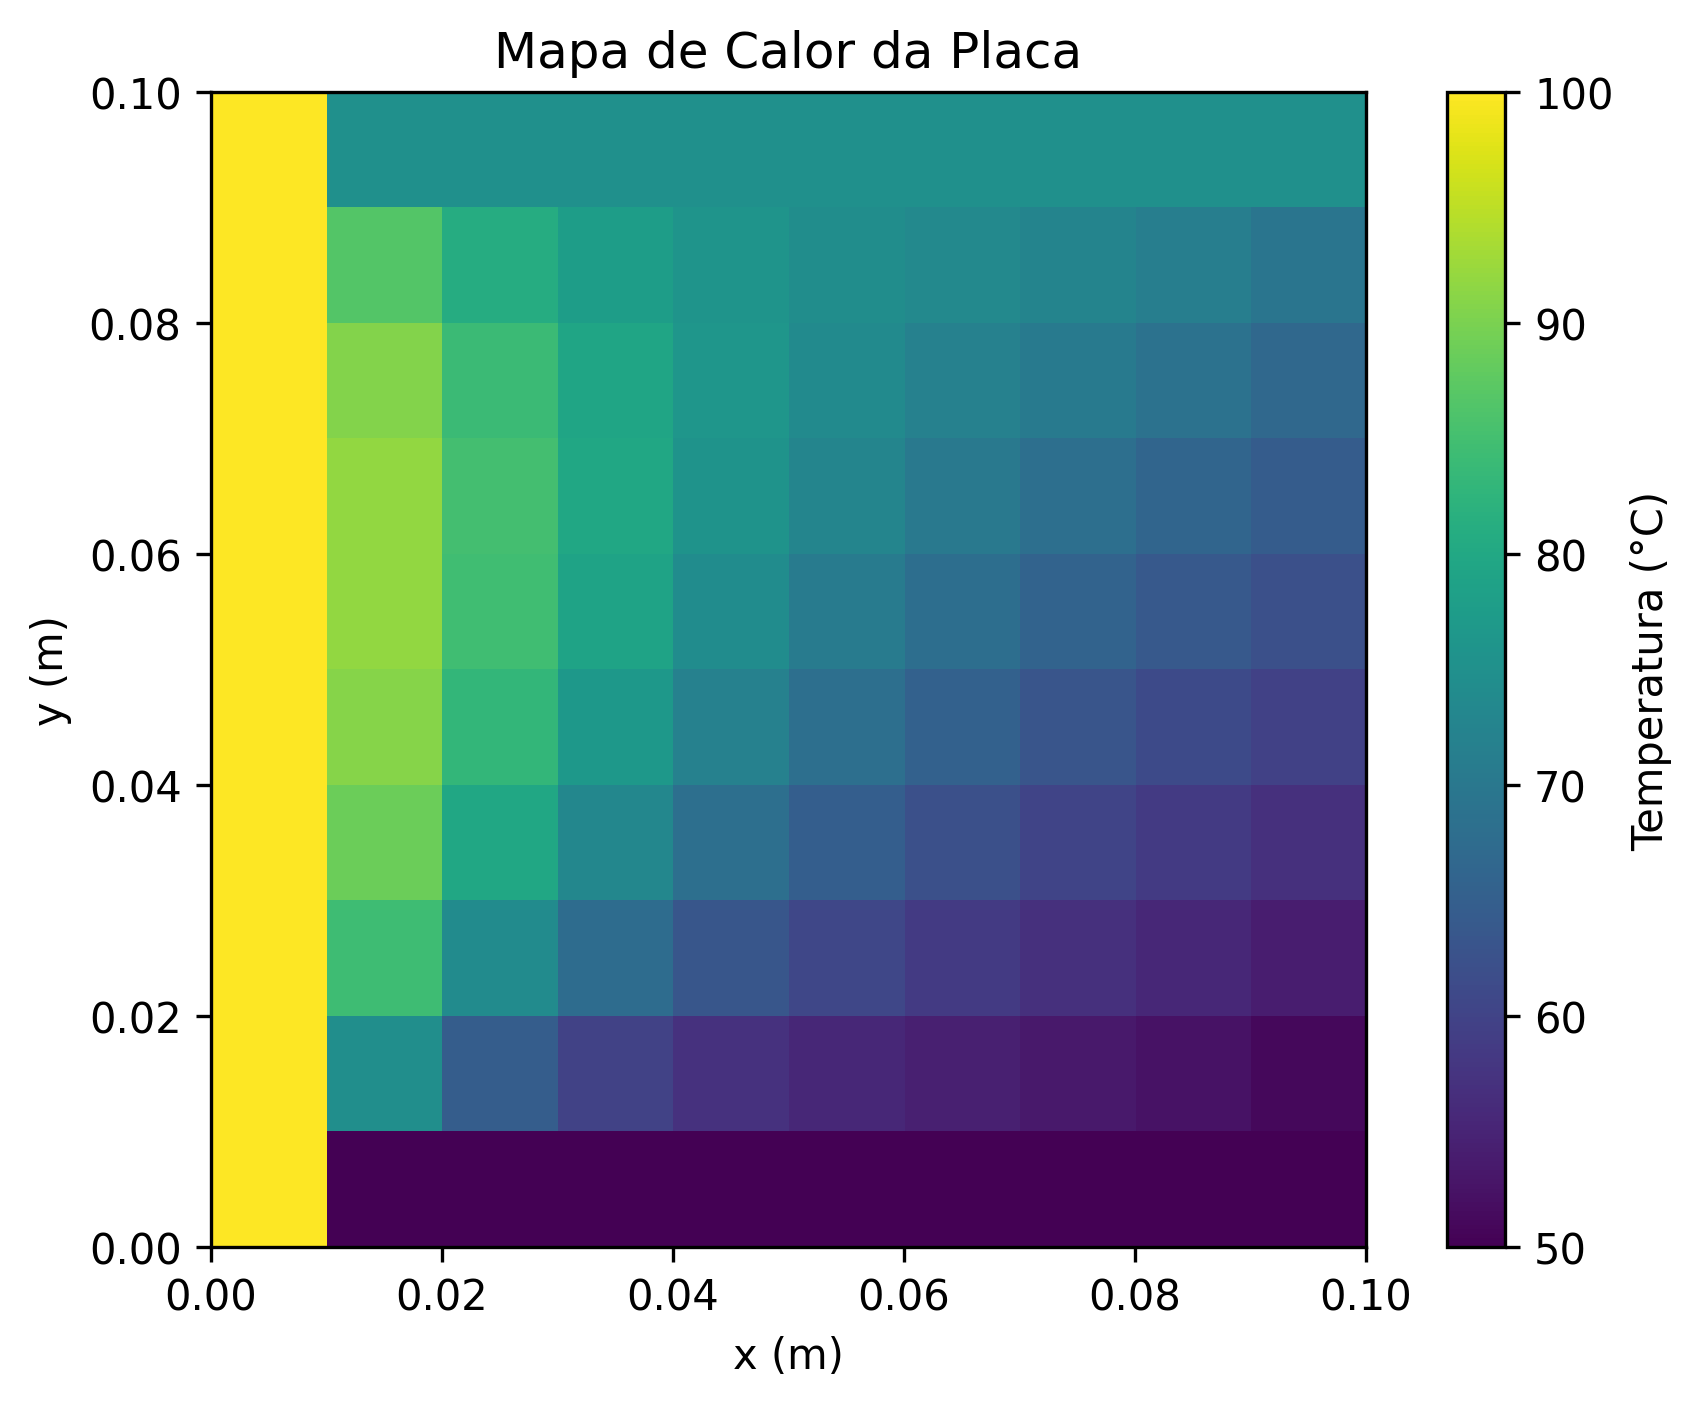
\includegraphics[width=0.7\linewidth]{mapa_calor.png}
    \caption{Mapa de calor da distribuição de temperatura na placa}
    \label{fig:lista1-mapa-calor}

    {\small Fonte: elaborado pelo autor.\par}
\end{figure}

Na Figura~\ref{fig:lista1-mapa-calor}, as maiores temperaturas aparecem perto
da borda esquerda, mantida a
$100\,^\circ$C, e as menores, junto à borda inferior, a $50\,^\circ$C. A partir
da borda superior, fixada em $75\,^\circ$C, a temperatura cai em direção à
direita devido à convecção com o ambiente a $10\,^\circ$C.

A condução produz uma transição contínua entre as fronteiras, com gradientes
mais intensos nos cantos que unem temperaturas distintas. Como a malha tem
apenas $10 \times 10$ nós, as faixas de cor ficam marcadas; uma malha mais fina
forneceria um campo mais suave e preciso.

% 

\chapter{Lista 2 -- Questão 1}

\section{Enunciado}

Considere a equação escalar de conservação sem fonte:
\[
    u_t + f(u)_x = 0,
\]
com
\[
    f(u)=\frac{1}{2}u^2.
\]

\begin{enumerate}
    \item Interprete fisicamente o termo $f(u)$
    \item Escreva a forma integral da equação em um intervalo fixo $I=[\alpha, \beta]$
    \item Suponha $u(x,0) = u_0$. Verifique se a função constante $u(x, t) \equiv u_0$ satisfaz a equação e a condição inicial.
\end{enumerate}

\section{Item 1}

A função $f(u)$ é o \textbf{fluxo} de $u$: ela mede a taxa de passagem dessa
quantidade por uma posição do domínio.

Neste caso,
\[
    f(u)=\frac{1}{2}u^2,
\]
portanto, sua dependência em relação a $u$ é não linear.

\section{Item 2}

No intervalo fixo
\[
    I=[\alpha,\beta].
\]

A integração da equação fornece
\[
    \int_{\alpha}^{\beta}u_t(x,t)\,dx
    +
    \int_{\alpha}^{\beta}f(u(x,t))_x\,dx
    =
    0.
\]

Como $\alpha$ e $\beta$ são fixos, aplica-se a regra de Leibniz:
\[
    \int_{\alpha}^{\beta}u_t(x,t)\,dx
    =
    \frac{d}{dt}
    \int_{\alpha}^{\beta}u(x,t)\,dx.
\]

Pelo Teorema Fundamental do Cálculo,
\[
    \int_{\alpha}^{\beta}f(u(x,t))_x\,dx
    =
    f(u(\beta,t))-f(u(\alpha,t)).
\]

Desse modo,
\[
    \frac{d}{dt}
    \int_{\alpha}^{\beta}u(x,t)\,dx
    +
    f(u(\beta,t))
    -
    f(u(\alpha,t))
    =
    0.
\]

A forma integral é, portanto,
\[
    \boxed{
        \frac{d}{dt}
        \int_{\alpha}^{\beta}u(x,t)\,dx
        =
        f(u(\alpha,t))-f(u(\beta,t))
    }.
\]

Como
\[
    f(u)=\frac{1}{2}u^2,
\]
resulta em
\[
    \boxed{
        \frac{d}{dt}
        \int_{\alpha}^{\beta}u(x,t)\,dx
        =
        \frac{1}{2}u(\alpha,t)^2
        -
        \frac{1}{2}u(\beta,t)^2
    }.
\]

Logo, a variação da quantidade total no intervalo é dada pelo fluxo de entrada
em $x=\alpha$ menos o de saída em $x=\beta$.

\section{Item 3}

A condição inicial é
\[
    u(x,0)=u_0,
\]
com $u_0$ constante.

Toma-se
\[
    u(x,t)=u_0.
\]

Como a função não varia em $x$ nem em $t$,
\[
    u_t(x,t)=0
\]
e
\[
    f(u(x,t))
    =
    f(u_0)
    =
    \frac{1}{2}u_0^2.
\]

e, como $f(u_0)$ também não varia em $x$,
\[
    f(u(x,t))_x=0.
\]

Assim,
\[
    u_t+f(u)_x=0+0=0.
\]

Para $t=0$,
\[
    u(x,0)=u_0,
\]
o que também satisfaz a condição inicial.

Conclui-se que
\[
    \boxed{u(x,t)=u_0}
\]
é a solução constante do problema.

\newpage

\chapter{Lista 3 -- Questão 1}

\section{Enunciado}

Considere a seguinte equação diferencial parcial hiperbólica não homogênea:

\[
    \frac{\partial u}{\partial t}
    +
    3\frac{\partial u}{\partial x}
    =
    1,
    \qquad x \in \mathbb{R}, \quad t>0,
\]

sujeita à condição inicial

\[
    u(x,0)=x^2,
    \qquad x\in\mathbb{R}.
\]

Pede-se:

\begin{enumerate}
    \item apresentar a solução da EDP hiperbólica não homogênea;
    \item representar graficamente as ondas formadas para diferentes valores de $t$;
    \item realizar a análise física das ondas obtidas.
\end{enumerate}

\section{Solução}

A equação tem a forma

\[
    u_t+a u_x=f,
\]

com velocidade de transporte constante

\[
    a=3,
\]

e fonte

\[
    f=1.
\]

Pelo método das características, considera-se uma curva $x=x(t)$. Nela, a
regra da cadeia fornece

\[
    \frac{d}{dt}u(x(t),t)
    =
    u_t
    +
    \frac{dx}{dt}u_x.
\]

Para coincidir com a EDP, define-se

\[
    \frac{dx}{dt}=3.
\]

Se a característica parte de $x_0$ em $t=0$, a integração resulta em

\[
    x(t)=x_0+3t.
\]

Logo,

\[
    x_0=x-3t.
\]

Ao longo de cada característica, resta a EDO

\[
    \frac{du}{dt}=1.
\]

Sua integração dá

\[
    u=t+C.
\]

A condição inicial determina $C$:

\[
    u(x_0,0)=x_0^2,
\]

assim,

\[
    C=x_0^2.
\]

Em cada característica,

\[
    u(x,t)=x_0^2+t.
\]

Substituindo $x_0=x-3t$, obtém-se:

\[
    \boxed{
        u(x,t)=(x-3t)^2+t
    }.
\]

A condição inicial é satisfeita, pois

\[
    u(x,0)
    =
    (x-3\cdot 0)^2+0
    =
    x^2.
\]

Para verificar a EDP, calculam-se

\[
    u_t=-6(x-3t)+1
\]

e

\[
    u_x=2(x-3t).
\]

Logo,

\[
    u_t+3u_x
    =
    -6(x-3t)+1+6(x-3t)
    =
    1.
\]

Portanto, a expressão satisfaz a EDP e a condição inicial.

\subsection{Implementação da solução}

No código, a solução é definida por

\begin{lstlisting}[language=Python]
def u(x, t):
    return (x - 3 * t) ** 2 + t
\end{lstlisting}

O intervalo espacial $[-10,20]$ é dividido em mil pontos:

\begin{lstlisting}[language=Python]
x = np.linspace(-10, 20, 1000)
\end{lstlisting}

Consideram-se os instantes

\[
    t=0,\quad 1,\quad 2,\quad 3,\quad 4.
\]

Para cada um deles, calcula-se e representa-se $u(x,t)$:

\begin{lstlisting}[language=Python]
tempos = [0, 1, 2, 3, 4]

for t in tempos:
    plt.plot(x, u(x, t), label=f"t = {t}")
\end{lstlisting}

\subsection{Perfis da solução}

\begin{figure}[H]
    \centering
    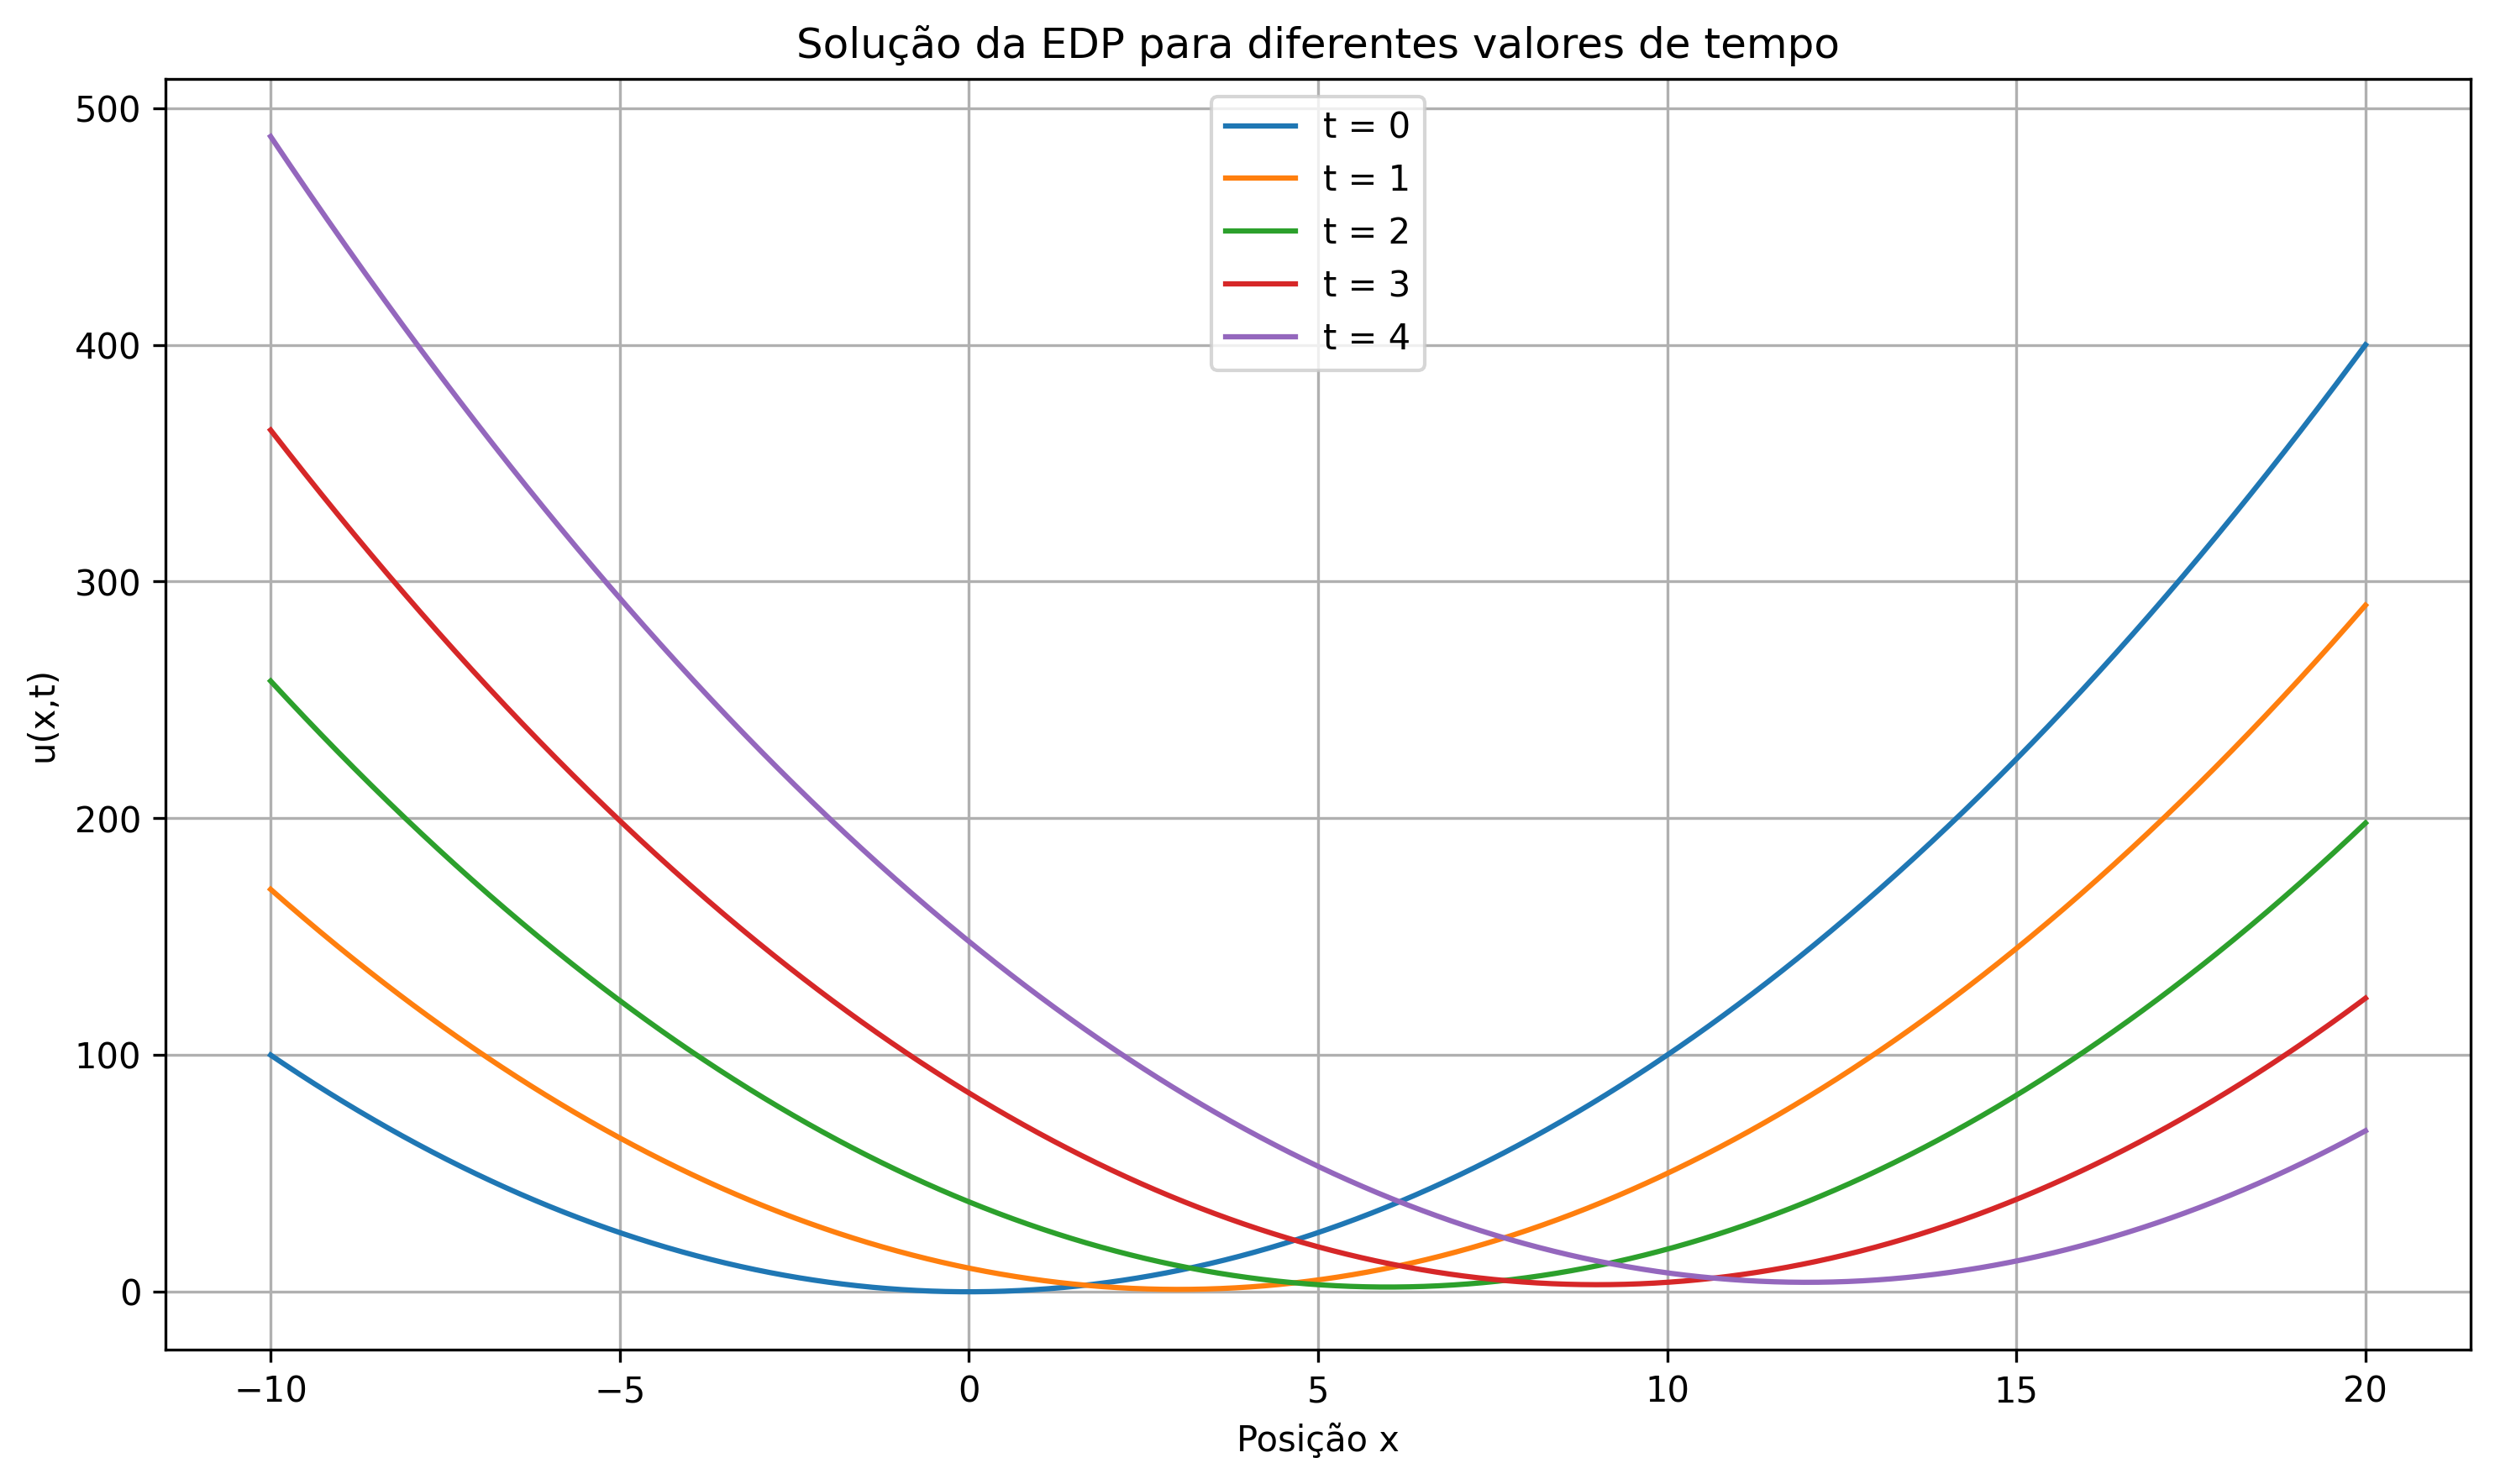
\includegraphics[width=0.85\linewidth]
    {01_solucao_edp.png}
    \caption{Solução da EDP para diferentes valores de tempo}
    \label{fig:lista3-perfis}

    {\small Fonte: elaborado pelo autor.\par}
\end{figure}

Na Figura~\ref{fig:lista3-perfis}, cada instante corresponde a uma parábola:

\[
    u(x,t)=(x-3t)^2+t.
\]

O vértice ocorre quando

\[
    x-3t=0.
\]

Sua posição e seu valor mínimo são, respectivamente,

\[
    x_{\mathrm{v}}=3t
\]

e

\[
    u_{\mathrm{v}}=t.
\]

A tabela resume o deslocamento do vértice:

\begin{table}[H]
    \centering
    \caption{Posição e valor do vértice em diferentes instantes}
    \label{tab:lista3-vertices}
    \begin{tabular}{ccc}
        \hline
        $t$ & $x_{\mathrm{v}}=3t$ & $u_{\mathrm{v}}=t$ \\
        \hline
        0   & 0                   & 0                  \\
        1   & 3                   & 1                  \\
        2   & 6                   & 2                  \\
        3   & 9                   & 3                  \\
        4   & 12                  & 4                  \\
        \hline
    \end{tabular}
\end{table}

\subsection{Representação tridimensional}

Para a visualização tridimensional, constrói-se uma malha em $x$ e $t$:

\begin{lstlisting}[language=Python]
x_superficie = np.linspace(-10, 20, 300)
t_superficie = np.linspace(0, 5, 200)

X, T = np.meshgrid(x_superficie, t_superficie)
U = u(X, T)
\end{lstlisting}

A matriz $U$ reúne a solução nos pontos da malha e define a superfície:

\begin{lstlisting}[language=Python]
fig = plt.figure(figsize=(11, 7))
ax = fig.add_subplot(111, projection="3d")

superficie = ax.plot_surface(
    X,
    T,
    U,
    cmap="viridis"
)
\end{lstlisting}

\begin{figure}[H]
    \centering
    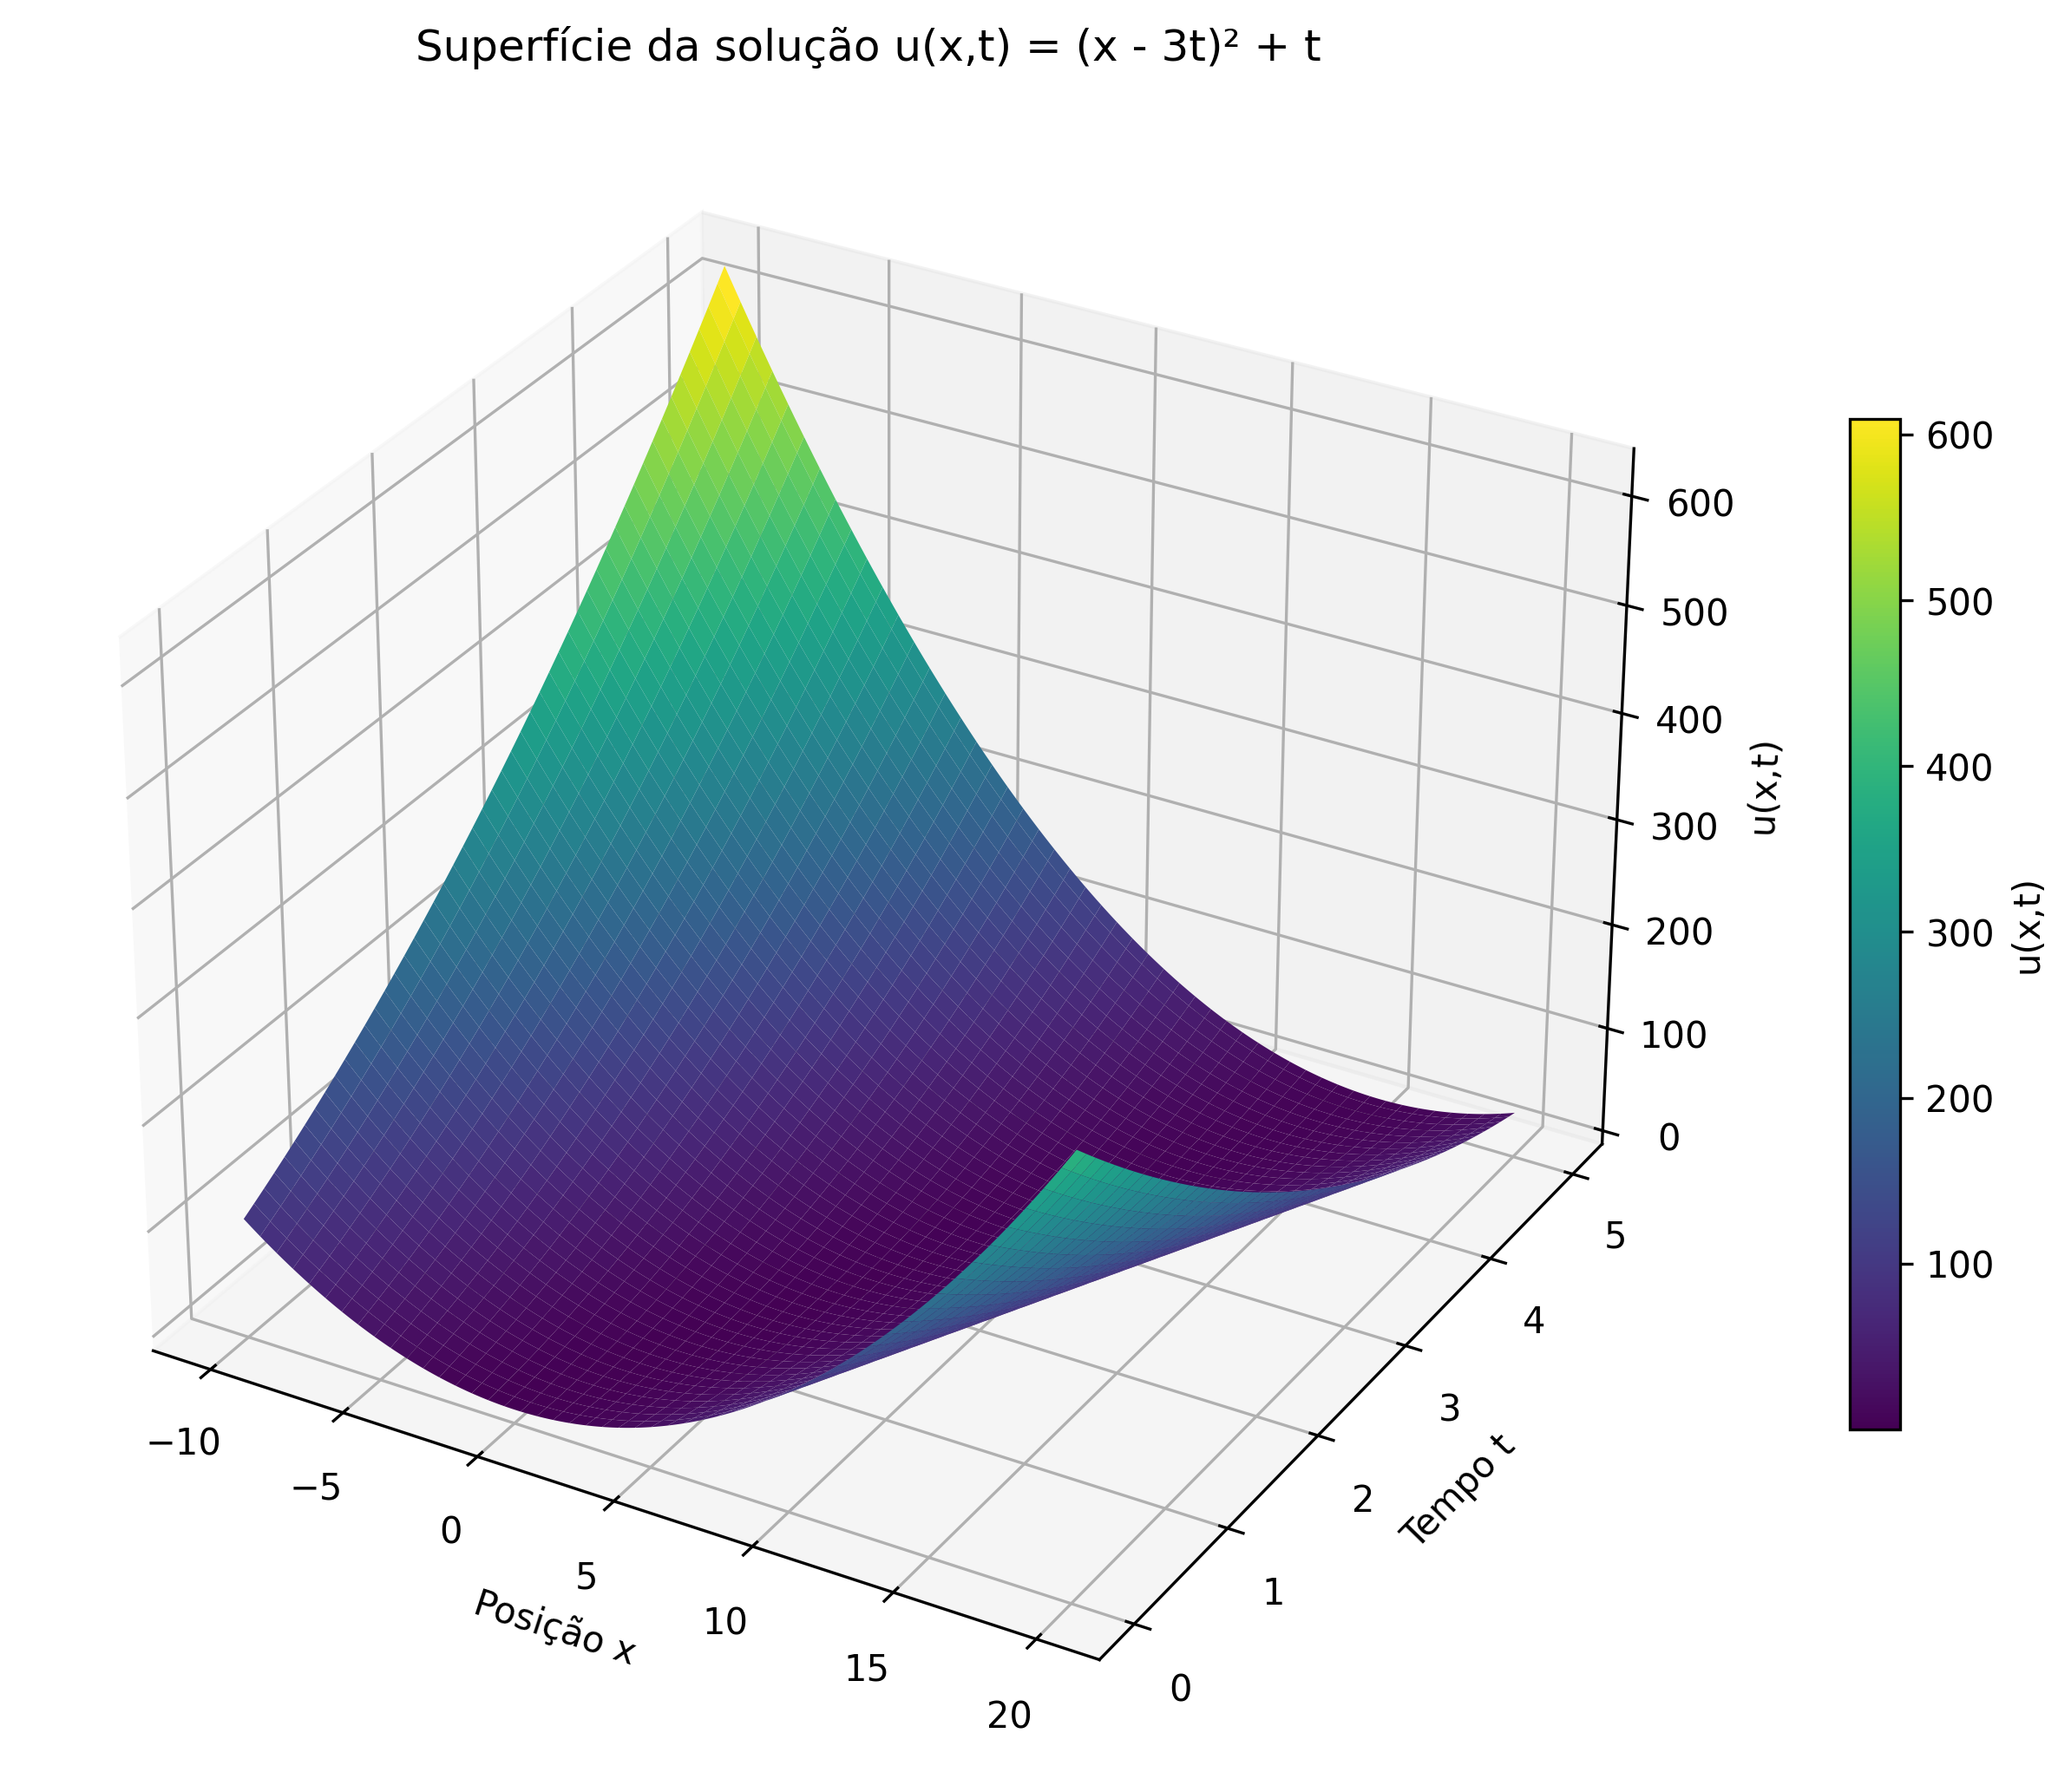
\includegraphics[width=0.85\linewidth]
    {02_representacao_grafica.png}
    \caption{Representação tridimensional da solução $u(x,t)$}
    \label{fig:lista3-superficie}

    {\small Fonte: elaborado pelo autor.\par}
\end{figure}

A Figura~\ref{fig:lista3-superficie} reúne a evolução dos perfis: $x$ indica a
posição, $t$ o tempo e o eixo vertical o valor de $u(x,t)$.

\subsection{Análise física}

O termo de transporte

\[
    3u_x
\]

desloca o perfil para a direita com velocidade constante $3$.

O termo $(x-3t)^2$ representa o deslocamento horizontal do perfil inicial
$x^2$. Em um tempo $t$, cada ponto percorre

\[
    \Delta x=3t.
\]

A fonte constante $1$ acrescenta $t$ à solução. Assim, enquanto se desloca para
a direita, a parábola também sobe uniformemente.

A forma e a abertura permanecem iguais porque todas as características têm a
mesma velocidade:

\[
    x=x_0+3t.
\]

Como essas retas são paralelas, não há cruzamentos, choques ou
descontinuidades.

Em síntese, há dois efeitos:

\begin{enumerate}
    \item deslocamento da parábola para a direita com velocidade $3$;
    \item elevação uniforme de uma unidade por unidade de tempo.
\end{enumerate}

\newpage

\chapter{Lista 3 -- Questão 2}

\section{Enunciado}

Considere a seguinte equação diferencial parcial hiperbólica homogênea:

\[
    \frac{\partial u}{\partial t}
    +
    a(x,t)\frac{\partial u}{\partial x}
    =
    0,
    \qquad x\in\mathbb{R}, \quad t>0,
\]

sujeita à condição inicial

\[
    u(x,0)=u_0(x),
    \qquad x\in\mathbb{R}.
\]

Pede-se:

\begin{enumerate}
    \item apresentar a solução da EDP hiperbólica homogênea;
    \item representar graficamente as ondas formadas para diferentes valores de $t$;
    \item realizar a análise física das ondas obtidas.
\end{enumerate}

\section{Solução}

A equação considerada possui a forma

\[
    u_t+a(x,t)u_x=0.
\]

O coeficiente $a(x,t)$ representa a velocidade de transporte da informação.
Diferentemente do caso em que a velocidade é constante, ela pode depender da
posição $x$ e do tempo $t$.

Pelo método das características, considera-se uma curva

\[
    x=X(t;x_0),
\]

que parte do ponto $x_0$ no instante inicial:

\[
    X(0;x_0)=x_0.
\]

Ao longo dessa curva, a regra da cadeia fornece

\[
    \frac{d}{dt}u(X(t;x_0),t)
    =
    u_t(X(t;x_0),t)
    +
    \frac{dX}{dt}u_x(X(t;x_0),t).
\]

Para que essa expressão coincida com a EDP, define-se a equação
característica

\[
    \frac{dX}{dt}
    =
    a(X(t;x_0),t).
\]

Dessa maneira,

\[
    \frac{d}{dt}u(X(t;x_0),t)
    =
    u_t+a(x,t)u_x.
\]

Como a equação é homogênea,

\[
    u_t+a(x,t)u_x=0,
\]

obtém-se

\[
    \frac{d}{dt}u(X(t;x_0),t)=0.
\]

Portanto, a solução permanece constante ao longo de cada curva
característica:

\[
    u(X(t;x_0),t)
    =
    u(X(0;x_0),0).
\]

Como

\[
    X(0;x_0)=x_0
\]

e a condição inicial é

\[
    u(x_0,0)=u_0(x_0),
\]

segue que

\[
    u(X(t;x_0),t)=u_0(x_0).
\]

Para determinar a solução em um ponto $(x,t)$, deve-se encontrar o ponto
inicial $x_0$ da característica que passa por esse ponto.

Se a relação

\[
    x=X(t;x_0)
\]

puder ser invertida em relação a $x_0$, escreve-se

\[
    x_0=X^{-1}(x,t).
\]

Assim, a solução geral é

\[
    \boxed{
        u(x,t)=u_0\left(X^{-1}(x,t)\right)
    }.
\]

Essa expressão mostra que o valor de $u$ em $(x,t)$ é determinado pelo valor
inicial localizado no ponto de origem da característica.

\subsection{Caso particular: velocidade constante}

Como o enunciado não fornece uma expressão específica para $a(x,t)$ nem para
$u_0(x)$, não é possível produzir um único gráfico numérico para o problema
geral.

Para ilustrar graficamente o comportamento da solução, considera-se o caso
particular

\[
    a(x,t)=c,
\]

em que $c$ é uma constante.

A equação característica torna-se

\[
    \frac{dX}{dt}=c.
\]

Integrando e utilizando a condição

\[
    X(0;x_0)=x_0,
\]

obtém-se

\[
    X(t;x_0)=x_0+ct.
\]

Logo,

\[
    x=x_0+ct
\]

e, isolando $x_0$,

\[
    x_0=x-ct.
\]

Como $u$ é constante ao longo das características,

\[
    u(x,t)=u_0(x_0).
\]

Substituindo $x_0=x-ct$, resulta em

\[
    \boxed{
        u(x,t)=u_0(x-ct)
    }.
\]

Portanto, quando a velocidade é constante, a solução corresponde a uma
translação do perfil inicial.

\subsection{Exemplo utilizado na representação gráfica}

Para a construção dos gráficos, considera-se

\[
    c=2
\]

e o perfil inicial

\[
    u_0(x)=e^{-x^2}.
\]

A EDP utilizada no exemplo é, portanto,

\[
    u_t+2u_x=0,
\]

com condição inicial

\[
    u(x,0)=e^{-x^2}.
\]

Aplicando a solução do caso constante,

\[
    u(x,t)=u_0(x-2t),
\]

obtém-se

\[
    \boxed{
        u(x,t)=e^{-(x-2t)^2}
    }.
\]

A condição inicial é satisfeita, pois

\[
    u(x,0)
    =
    e^{-(x-2\cdot 0)^2}
    =
    e^{-x^2}.
\]

Para verificar a EDP, calculam-se as derivadas

\[
    u_t
    =
    4(x-2t)e^{-(x-2t)^2}
\]

e

\[
    u_x
    =
    -2(x-2t)e^{-(x-2t)^2}.
\]

Logo,

\[
    u_t+2u_x
    =
    4(x-2t)e^{-(x-2t)^2}
    -
    4(x-2t)e^{-(x-2t)^2}
    =
    0.
\]

Portanto, a expressão satisfaz a EDP e a condição inicial.

\subsection{Implementação da solução}

No código, o perfil inicial é definido por

\begin{lstlisting}[language=Python]
def u0(x):
    return np.exp(-x**2)
\end{lstlisting}

A solução é implementada por

\begin{lstlisting}[language=Python]
def u(x, t, c=2):
    return u0(x - c * t)
\end{lstlisting}

O intervalo espacial $[-10,15]$ é dividido em mil pontos:

\begin{lstlisting}[language=Python]
x = np.linspace(-10, 15, 1000)
\end{lstlisting}

São considerados os instantes

\[
    t=0,\quad 1,\quad 2,\quad 3,\quad 4.
\]

Para cada instante, calcula-se e representa-se o perfil da solução:

\begin{lstlisting}[language=Python]
tempos = [0, 1, 2, 3, 4]

for t in tempos:
    plt.plot(x, u(x, t), label=f"t = {t}")
\end{lstlisting}

\subsection{Perfis da solução}

\begin{figure}[H]
    \centering
    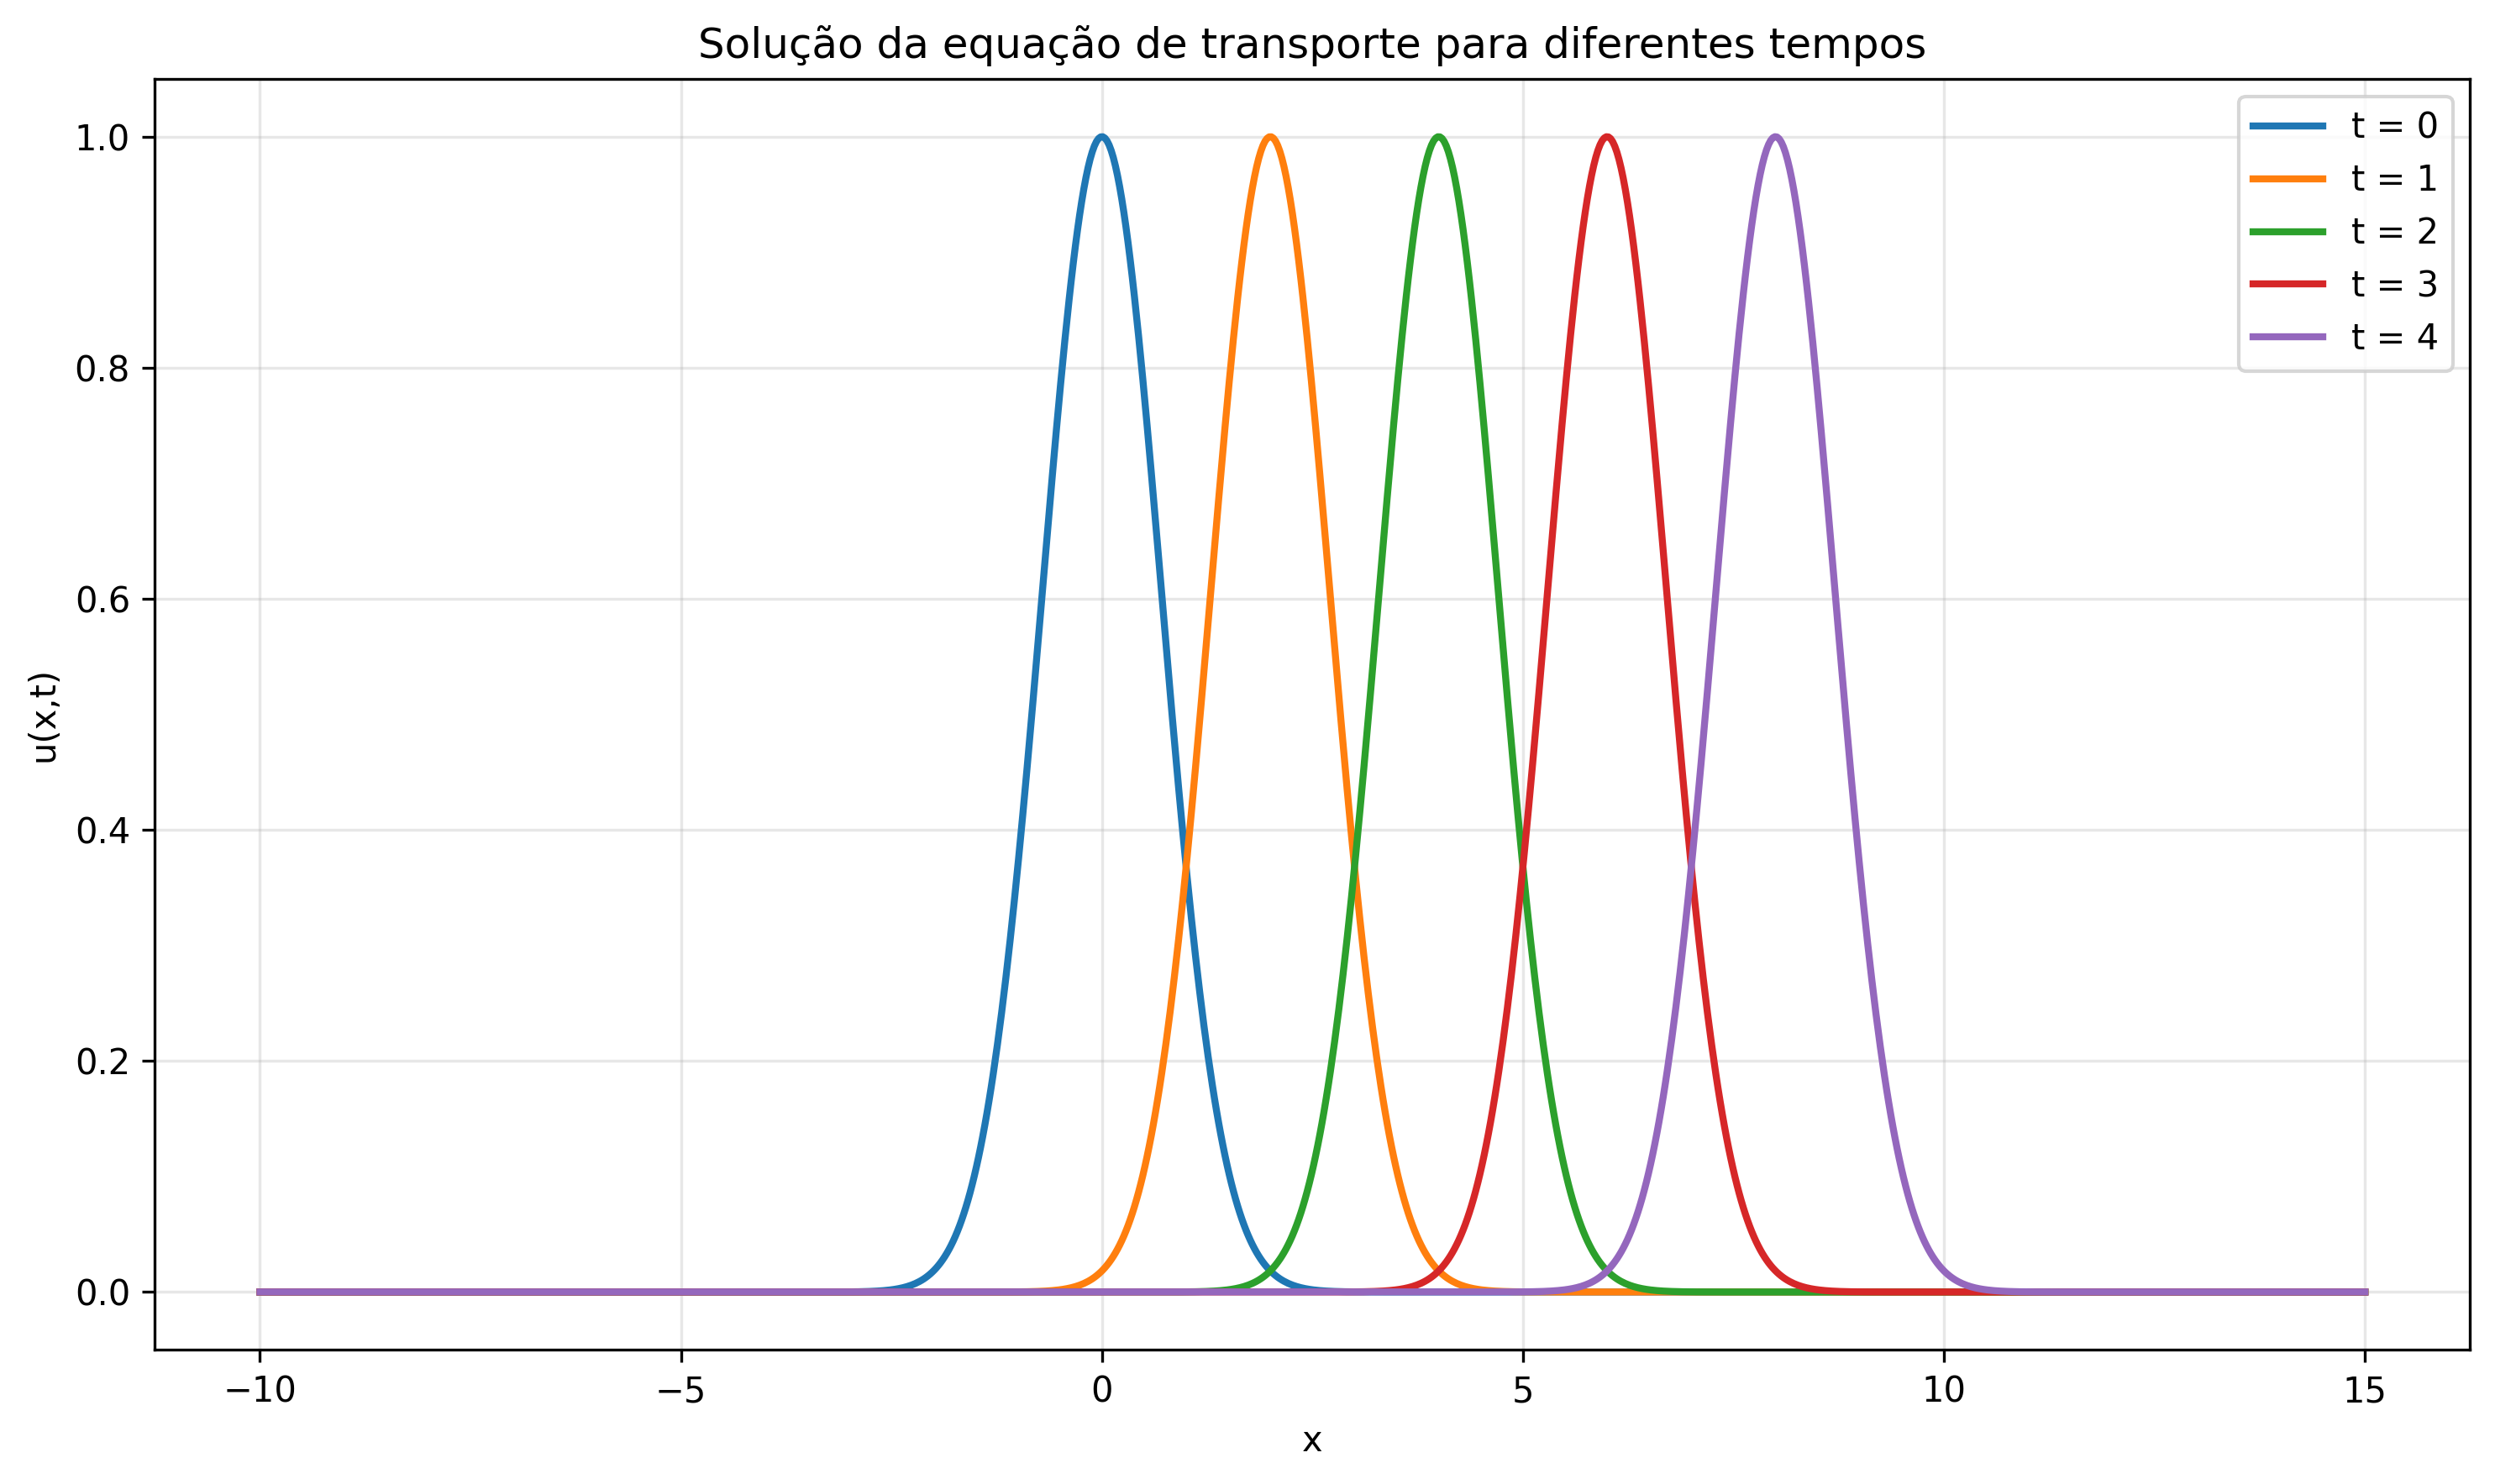
\includegraphics[width=0.85\linewidth]
    {03_solucao_questao2.png}
    \caption{Solução da equação de transporte para diferentes valores de tempo}
    \label{fig:lista3-questao2-perfis}

    {\small Fonte: elaborado pelo autor.\par}
\end{figure}

Na Figura~\ref{fig:lista3-questao2-perfis}, cada instante corresponde ao
perfil

\[
    u(x,t)=e^{-(x-2t)^2}.
\]

O valor máximo da função ocorre quando

\[
    x-2t=0.
\]

Portanto, a posição do máximo é

\[
    x_{\mathrm{m}}=2t.
\]

O valor máximo permanece igual a

\[
    u_{\mathrm{m}}=1.
\]

A tabela resume o deslocamento do centro do perfil:

\begin{table}[H]
    \centering
    \caption{Posição e valor máximo do perfil em diferentes instantes}
    \label{tab:lista3-questao2-maximos}
    \begin{tabular}{ccc}
        \hline
        $t$ & $x_{\mathrm{m}}=2t$ & $u_{\mathrm{m}}$ \\
        \hline
        0   & 0                   & 1                \\
        1   & 2                   & 1                \\
        2   & 4                   & 1                \\
        3   & 6                   & 1                \\
        4   & 8                   & 1                \\
        \hline
    \end{tabular}
\end{table}

\subsection{Mapa das características}

No caso de velocidade constante $c=2$, as curvas características são dadas
por

\[
    x=x_0+2t.
\]

Essas curvas podem ser representadas no plano formado pela posição $x$ e pelo
tempo $t$.

\begin{lstlisting}[language=Python]
x0_valores = np.linspace(-8, 8, 17)
t_caracteristicas = np.linspace(0, 5, 300)

for x0 in x0_valores:
    x_caracteristica = x0 + 2 * t_caracteristicas
    plt.plot(
        x_caracteristica,
        t_caracteristicas
    )
\end{lstlisting}

\begin{figure}[H]
    \centering
    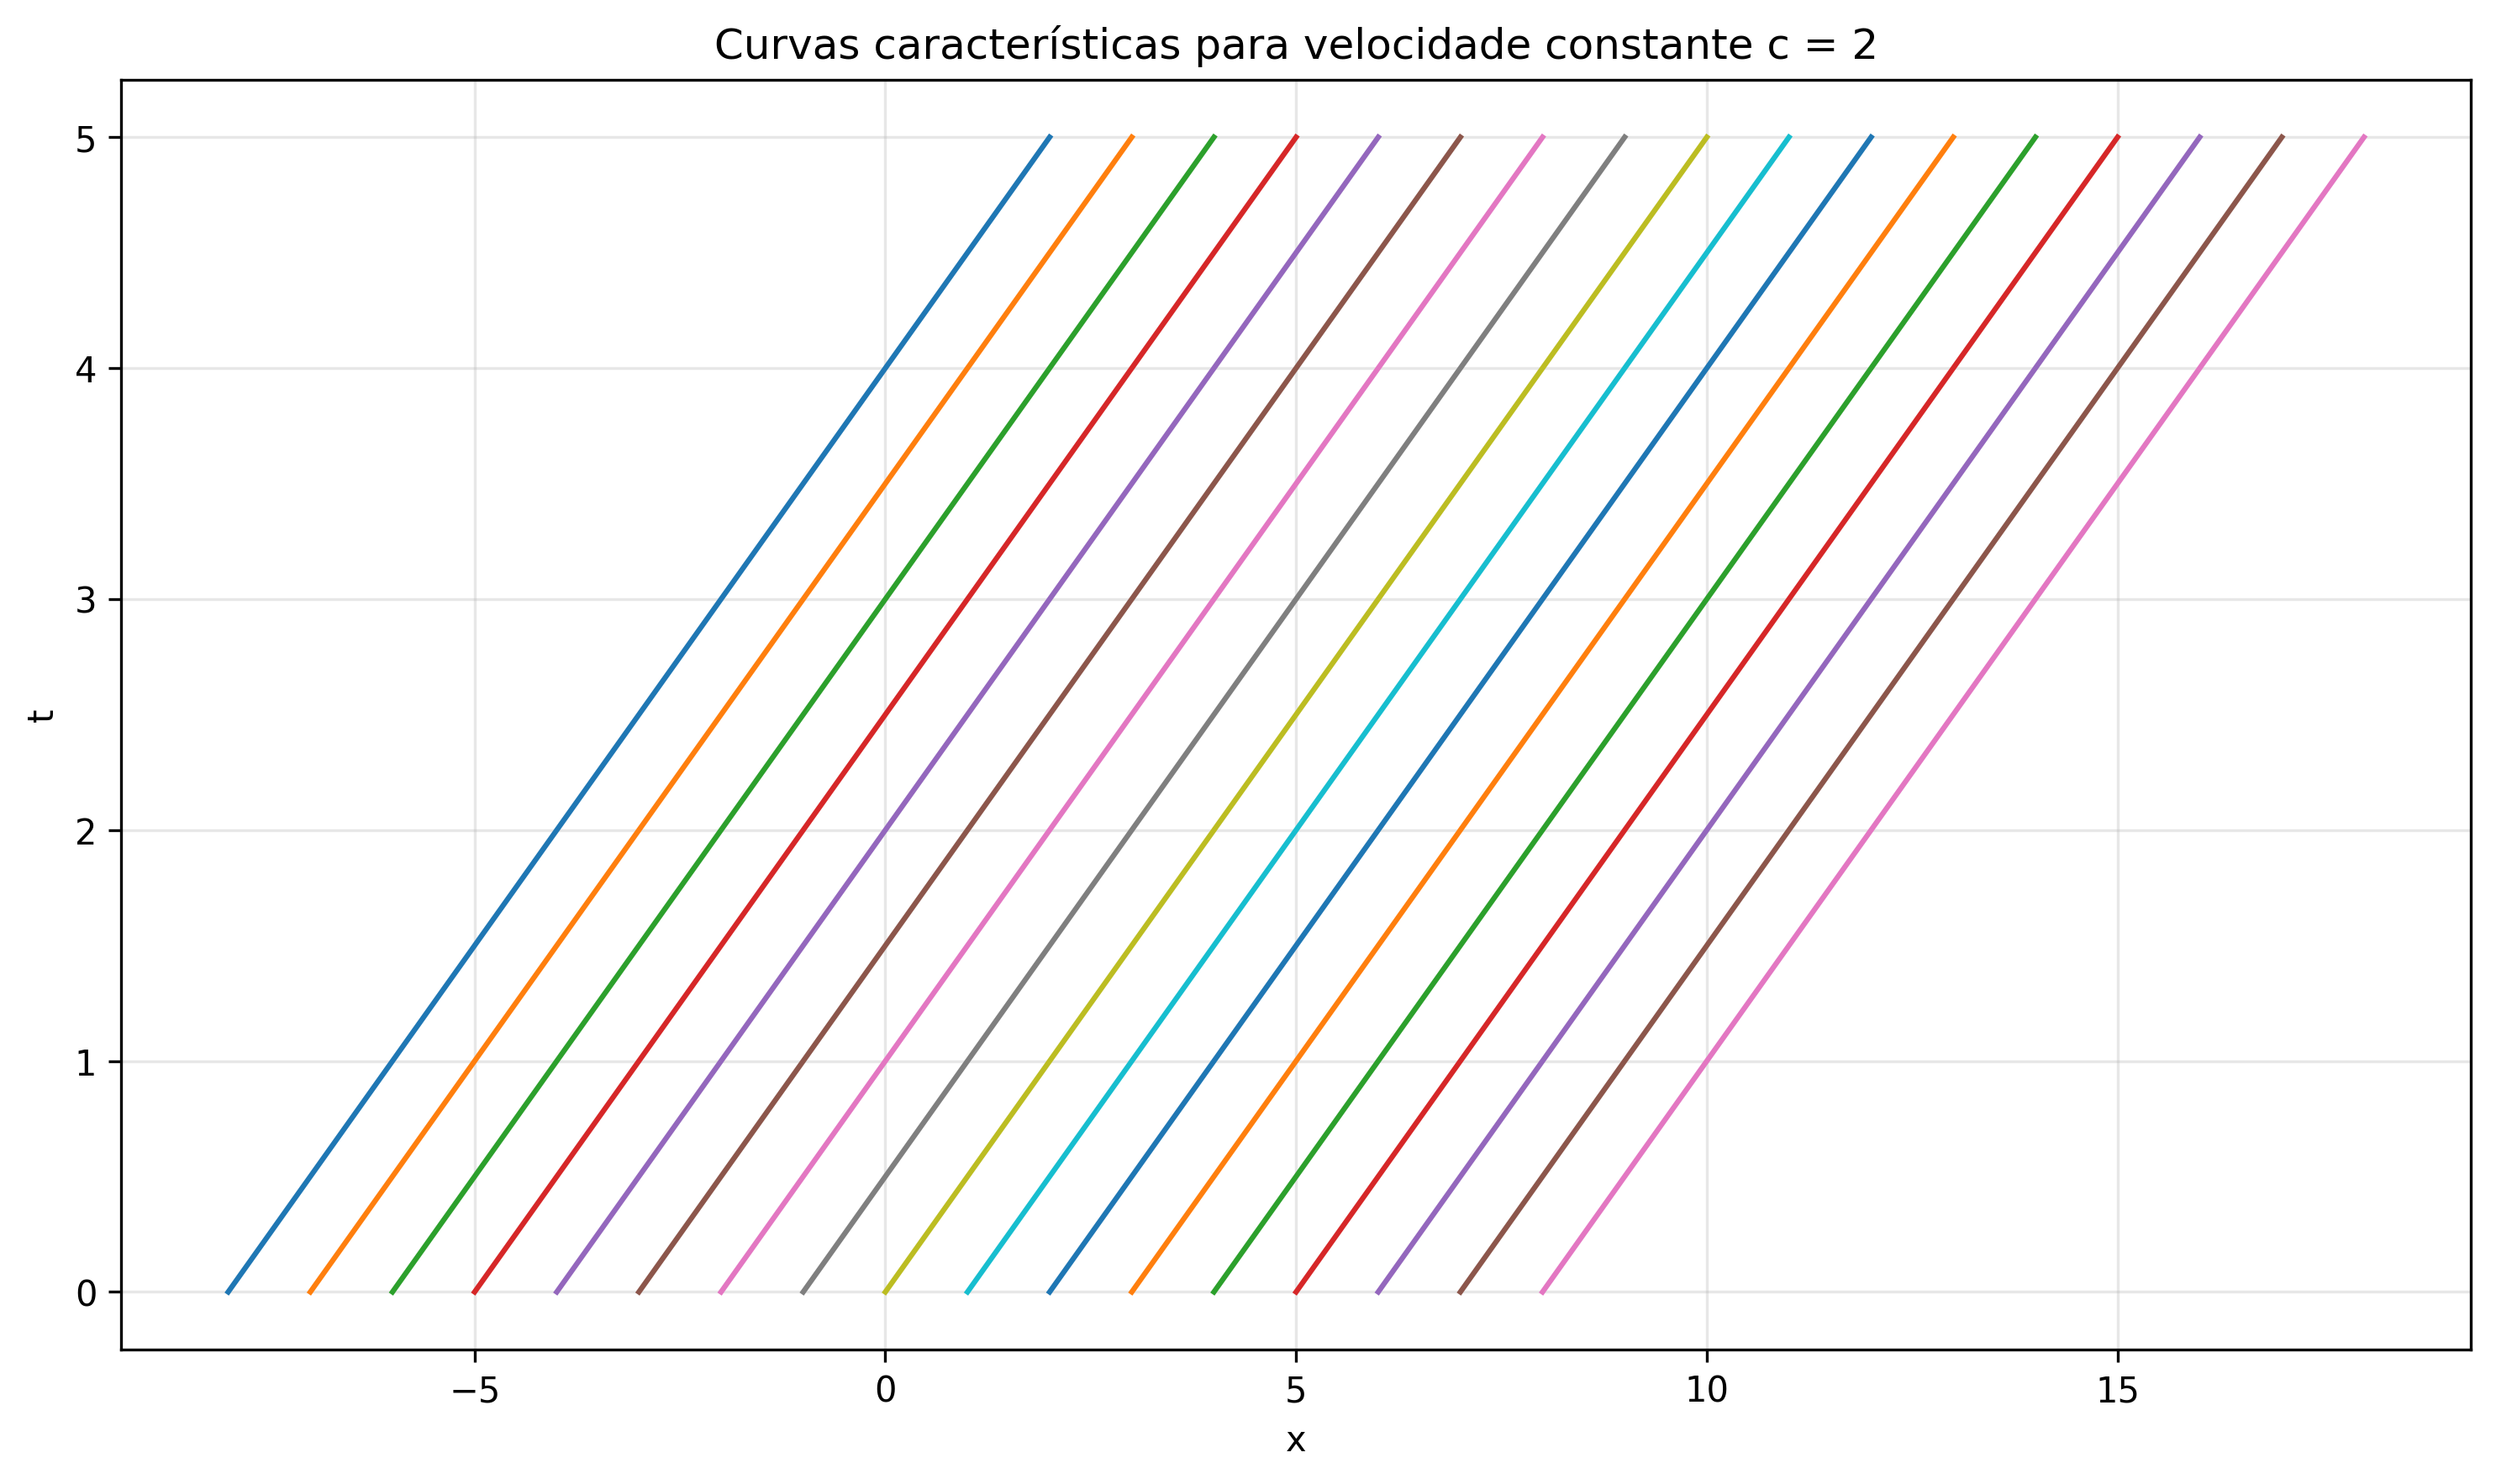
\includegraphics[width=0.85\linewidth]
    {04_caracteristicas_questao2.png}
    \caption{Curvas características para velocidade constante $c=2$}
    \label{fig:lista3-questao2-caracteristicas}

    {\small Fonte: elaborado pelo autor.\par}
\end{figure}

Na Figura~\ref{fig:lista3-questao2-caracteristicas}, as características são
retas paralelas porque todas possuem a mesma velocidade.

Um ponto que inicia na posição $x_0$ segue a trajetória

\[
    x=x_0+2t.
\]

Ao longo dessa trajetória, o valor de $u$ permanece constante:

\[
    u(x_0+2t,t)=u_0(x_0).
\]

\subsection{Representação tridimensional}

Para visualizar simultaneamente a dependência da solução em relação a $x$ e
$t$, constrói-se uma malha:

\begin{lstlisting}[language=Python]
x_superficie = np.linspace(-10, 15, 300)
t_superficie = np.linspace(0, 5, 200)

X, T = np.meshgrid(x_superficie, t_superficie)
U = u(X, T)
\end{lstlisting}

A superfície é construída por

\begin{lstlisting}[language=Python]
fig = plt.figure(figsize=(11, 7))
ax = fig.add_subplot(111, projection="3d")

superficie = ax.plot_surface(
    X,
    T,
    U,
    cmap="viridis"
)
\end{lstlisting}

\begin{figure}[H]
    \centering
    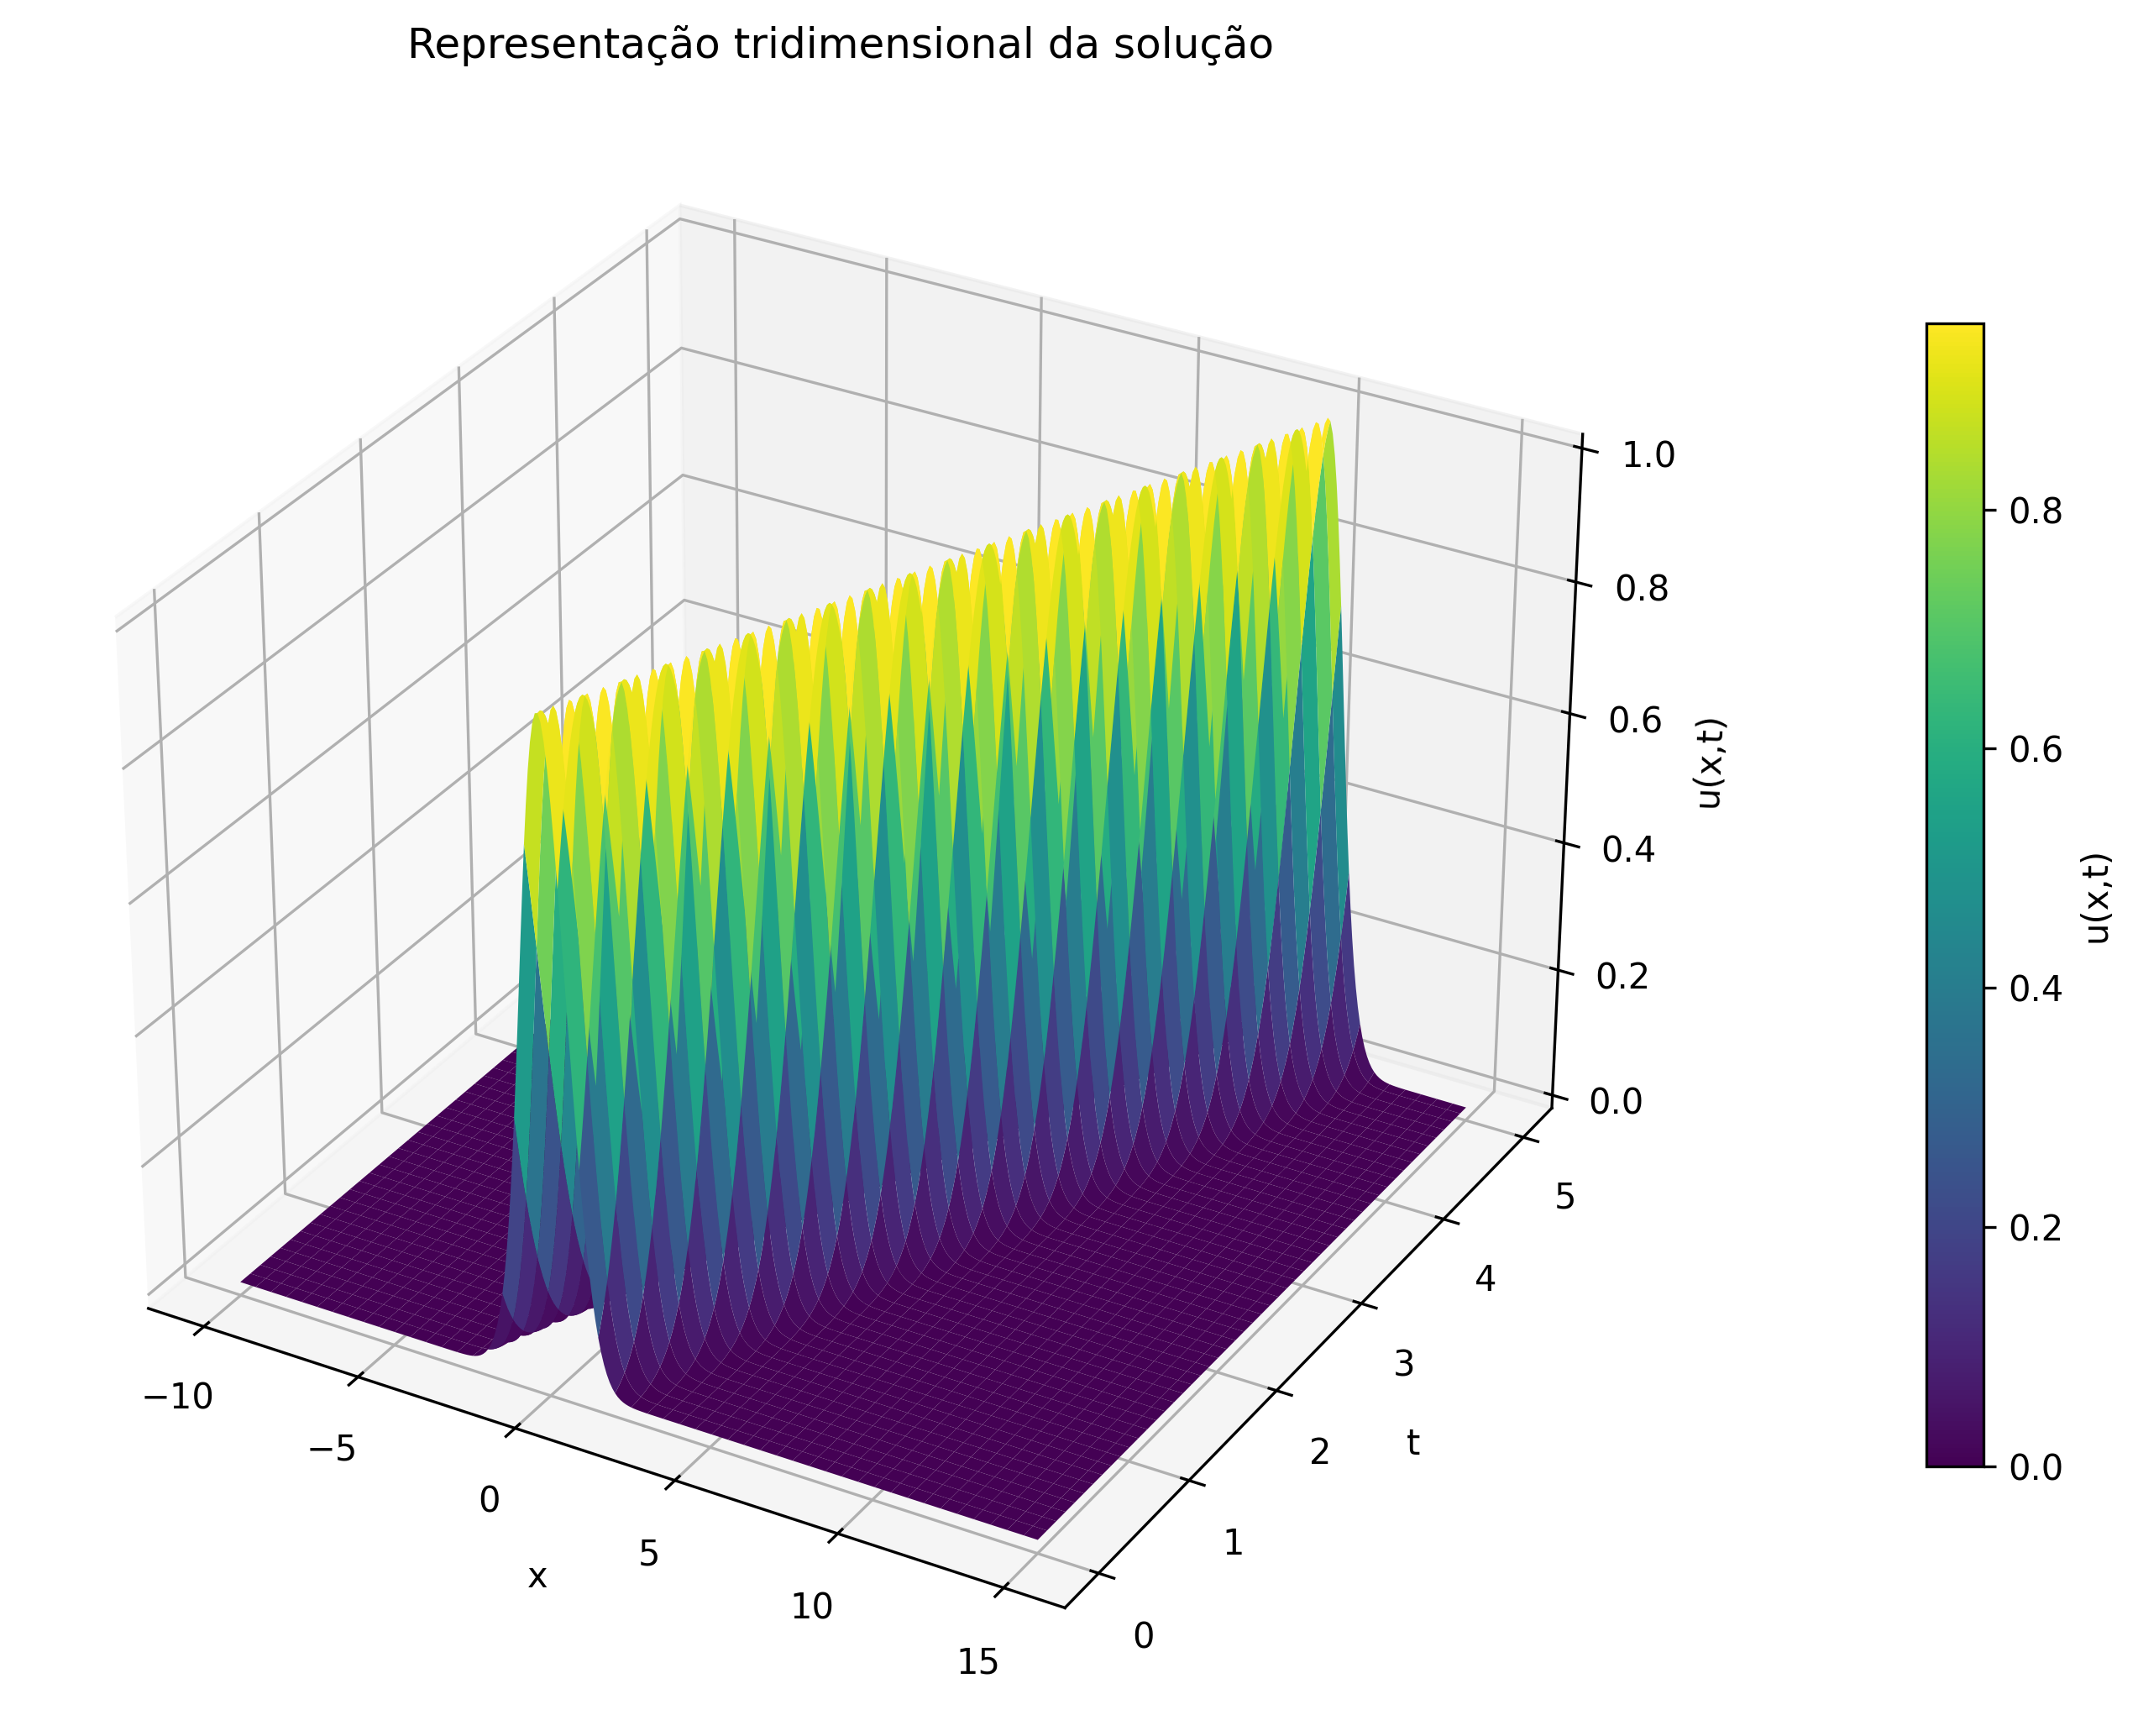
\includegraphics[width=0.85\linewidth]
    {05_superficie_questao2.png}
    \caption{Representação tridimensional da solução $u(x,t)$}
    \label{fig:lista3-questao2-superficie}

    {\small Fonte: elaborado pelo autor.\par}
\end{figure}

A Figura~\ref{fig:lista3-questao2-superficie} reúne a evolução temporal dos
perfis. O eixo $x$ indica a posição, o eixo $t$ representa o tempo e o eixo
vertical corresponde ao valor de $u(x,t)$.

\subsection{Análise física}

A equação

\[
    u_t+a(x,t)u_x=0
\]

representa o transporte de uma quantidade sem a presença de fontes,
sumidouros ou termos difusivos.

O coeficiente $a(x,t)$ determina a velocidade local de propagação. Como a
equação é homogênea, o valor de $u$ não aumenta nem diminui ao longo de uma
característica:

\[
    \frac{du}{dt}=0.
\]

Isso significa que as características transportam os valores do perfil
inicial sem modificá-los diretamente.

No caso particular em que

\[
    a(x,t)=c,
\]

a solução é

\[
    u(x,t)=u_0(x-ct).
\]

Nesse caso, o perfil inicial sofre apenas uma translação horizontal.

Quando

\[
    c>0,
\]

a propagação ocorre da esquerda para a direita.

Quando

\[
    c<0,
\]

a propagação ocorre da direita para a esquerda.

Para o exemplo considerado,

\[
    c=2,
\]

o perfil desloca-se para a direita com velocidade constante igual a $2$.
Após um intervalo de tempo $t$, o deslocamento é

\[
    \Delta x=2t.
\]

A amplitude máxima permanece igual a $1$, e a largura e a forma do perfil não
são alteradas. Isso acontece porque todas as características possuem a mesma
velocidade e permanecem paralelas.

Consequentemente, no caso constante:

\begin{enumerate}
    \item o perfil desloca-se com velocidade constante;
    \item a forma da onda permanece inalterada;
    \item a amplitude permanece constante;
    \item não ocorre dissipação;
    \item não ocorre crescimento ou decaimento;
    \item não ocorre cruzamento das características;
    \item não ocorre formação de choques ou descontinuidades.
\end{enumerate}

No caso geral, em que $a=a(x,t)$, a velocidade pode variar entre diferentes
pontos do domínio. Assim, as características podem deixar de ser retas e o
perfil pode sofrer compressão ou expansão espacial.

Entretanto, enquanto as características não se cruzarem, a solução continua
sendo obtida transportando o dado inicial:

\[
    \boxed{
        u(x,t)=u_0\left(X^{-1}(x,t)\right)
    }.
\]

Em síntese, a equação descreve o transporte da informação inicial ao longo das
curvas determinadas pela velocidade $a(x,t)$, mantendo constante o valor da
solução sobre cada uma dessas trajetórias.

\postextual
\chapter*{Referências}
\addcontentsline{toc}{chapter}{REFERÊNCIAS}

LEVEQUE, Randall J. \textit{Numerical Methods for Conservation Laws}. Zürich:
Birkhäuser/ETH Zürich, 1990.

CUNHA, Maria Cristina C. \textit{Métodos Numéricos}. Campinas: Editora da
UNICAMP, 2000.

\end{document}
